\chapter{Hash Tables}
    
        \section{Static Hashing with Chaining}
    
        %Time complexity for item search, insert and delete: $\Theta(1)$.
    
        The model is based on the idea of having a universe of items, each with a distinct key.
        
        We define a hash function $h: \mathcal{U} \rightarrow [0, m-1]$ which will be used to map the items to our table. However, there might be collisions: $\exists k_i \neq k_j$ s.t. $h(k_i) = h(k_j)$.
        
        We need to make some assumptions in order to make it work:
    
        \begin{itemize}
            \item Each key of $\mathcal{U}$ is equally likely to be hashed to any slot of the hash table (\textbf{uniformity}). $Pr(h(k) = i) = \frac{1}{m} \forall k \in \mathcal{U}, \forall i \in [0, m-1]$
    
            \item Each key is mapped to a slot independently from the items already in the table (\textbf{independency}).
    
            \item $h(k)$ can be computed in $\Theta(1)$ time.\\
        \end{itemize}

        \vspace{-1em}

        \begin{figure}[H]
            \centering
            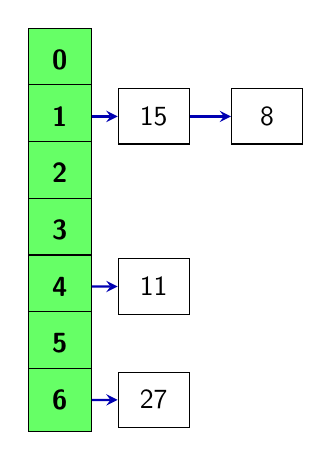
\begin{tikzpicture}[
                scale=0.8,
                node distance=0.8cm,
                every node/.style={font=\sffamily},
                hashcell/.style={rectangle, draw=black, fill=green!60, minimum width=0.8cm, minimum height=0.8cm, anchor=west},
                pointer/.style={-stealth, thick, draw=blue!70!black},
                valuebox/.style={rectangle, draw=black, minimum width=0.9cm, minimum height=0.7cm, fill=white}
            ]
                % Hash table cells
                \foreach \i in {0,...,6} {
                    \node[hashcell] (cell\i) at (0,-\i*0.9) {\textbf{\i}};
                }
                
                % Linked list nodes
                \node[valuebox] (v15) at (2,-0.9) {15};
                \node[valuebox] (v8)  at (3.8,-0.9) {8};
                \node[valuebox] (v11) at (2,-3.6) {11};
                \node[valuebox] (v27) at (2,-5.4) {27};
                
                % Pointers from hash table to first node
                \draw[pointer] (cell1.east) -- (v15.west);
                \draw[pointer] (cell4.east) -- (v11.west);
                \draw[pointer] (cell6.east) -- (v27.west);
                
                % Pointers for chaining
                \draw[pointer] (v15.east) -- (v8.west);
            \end{tikzpicture}
            \caption{Hash table with chaining containing 7 buckets (0-6). The keys 15, 11, 27, and 8 are inserted in sequence.}
            \label{fig:hash-table-chaining}
        \end{figure}

          \vspace{-1em}
        
        Suppose we have stored $n$ items into a table of size $m$. Then, the expected size of any list is $\frac{n}{m}$ (load factor $\alpha$).
        
        \begin{table}[H]
            \centering
            \begin{tabular}{ccc}
                 & \textbf{Expected Time} & \textbf{Worst Case Time}\\
                \textbf{Insert} & $\Theta(1)$ & $\Theta(1)$\\
                \textbf{Search} & $\Theta(1 + \alpha)$ & $\Theta(n)$\\
                \textbf{Delete} & $\Theta (1 + \alpha)$ & $\Theta(n)$\\
            \end{tabular}
            \label{tab:my_label}
            \caption{Operation complexity in a static hash table.}
        \end{table}

        The expected time to \textbf{search} for a key is $\Theta(1 + \frac{n}{m}) = \Theta(1+\alpha)$, that is equal to $\Theta(1)$ if $n=O(m)$ ($\frac{n}{m} = O(1)$). Worst case is $\Theta(n)$ (all elements go to the same slot). The \textbf{insert} time is $\Theta(1)$ worst case because it is only required to compute the hash function. 
        
        The \textbf{delete} expected time is $\Theta(1 + \frac{n}{m})$ (search + deletion). $\Theta(n)$ worst case.

        \section{Dynamic Hashing with Chaining}
    
        Dynamic hashing extends the static approach by allowing the hash table to grow and shrink dynamically based on the number of elements. This maintains optimal space utilization and performance.

        The key invariant is maintaining $m \geq n$, or more precisely, $\frac{n}{m} = \Theta(1)$; when inserting the $\small (m+1)$-th element into a table of size $m$, we create a new table of size $m' > m$. This process involves three steps:
    
        \begin{enumerate}
            \item Allocate a new hash table of size $m'$ in $\Theta(m')$ time
    
            \item Generate a new hash function $h':\mathcal{U} \rightarrow [0, m' - 1]$ in $\Theta(m')$ time
    
            \item Rehash all existing items into the new table using $h'$ in $\Theta(m + n)$ time
        \end{enumerate}
    
        For \textbf{growing} the table, we use a doubling strategy: $m' = 2m$. This choice of growth factor ensures optimal amortized performance.

        Consider inserting $n$ items sequentially into an initially empty table. The total cost is $\Theta(1+2+4+8+\dots+n) = \Theta(\sum_{i=0}^{\log n} 2^i) = \Theta(n)$, yielding an amortized cost of $\Theta(1)$ per operation.
        
        For \textbf{shrinking}, we follow a similar process:
    
        \begin{enumerate}
            \item Allocate a new table of size $m'$
    
            \item Generate a new hash function $h':\mathcal{U} \rightarrow [0, m' - 1]$
    
            \item Rehash all $n$ items into the new table
        \end{enumerate}
    
        We trigger shrinking when $n = \dfrac{m}{4}$, setting $m'=\dfrac{m}{2}$. This threshold of $\frac{1}{4}$ (rather than $\frac{1}{2}$) prevents thrashing between grow and shrink operations near the boundary.
        
        The total cost for growing or shrinking is $\Theta(m' + m + n)$.
        
        A crucial observation is that deletions can only occur for previously inserted items. Therefore, the total deletion cost is bounded by the total insertion cost of $\Theta(n)$, leading to an amortized cost of $\Theta(1)$ per operation.
    
        \begin{table}[H]
            \centering
            \begin{tabular}{ccc}
                 & \textbf{Expected Time} & \textbf{Worst Case Time}\\
                \textbf{Insert} & $\Theta(1)$ & $\Theta(m' + m + n)$\\
                \textbf{Search} & $\Theta(1 + \alpha)$ & $\Theta(n)$\\
                \textbf{Delete} & $\Theta (1 + \alpha)$ & $\Theta(m' + m + n)$\\
            \end{tabular}
            \label{tab:my_label}
            \caption{Operation complexity in a dynamic hash table.}
        \end{table}